\documentclass[a4paper,10pt]{article}
\usepackage[T1]{fontenc}
\usepackage[margin=1cm]{geometry}
\usepackage{tikz}
\usepackage{xcolor}
\renewcommand{\familydefault}{\rmdefault}
\pagestyle{empty}
% === Colour definitions ===
\definecolor{catTrauma}{HTML}{3B82B0}
\definecolor{catAnxiety}{HTML}{3B82B0}
\definecolor{catMood}{HTML}{3B82B0}
\definecolor{catOCD}{HTML}{3B82B0}
\definecolor{catOther}{HTML}{3B82B0}
\definecolor{catSomatic}{HTML}{3B82B0}
\definecolor{catEating}{HTML}{3B82B0}
\definecolor{catNeuro}{HTML}{3B82B0}
\definecolor{catPsychotic}{HTML}{3B82B0}
\definecolor{catPersonality}{HTML}{3B82B0}
\definecolor{catSelfHarm}{HTML}{3B82B0}
\definecolor{catSubstance}{HTML}{3B82B0}
\definecolor{catSleep}{HTML}{3B82B0}
\definecolor{catGold}{HTML}{E9C46A}
\definecolor{catUnclass}{HTML}{94A3B8}
\definecolor{sevCritical}{HTML}{9B2226}
\definecolor{sevSevere}{HTML}{E10600}
\definecolor{sevModerate}{HTML}{F07B83}
\definecolor{sevMild}{HTML}{F6C1C4}
\definecolor{studyA}{HTML}{3B82C4}
\definecolor{studyB}{HTML}{F4A261}
\definecolor{studyC}{HTML}{2A9D8F}
\definecolor{modTeal}{HTML}{3C8D93}
\definecolor{textdark}{HTML}{111827}
\definecolor{gridlight}{HTML}{D8DEE9}

\begin{document}
% Fig 3: Severity Distribution (donut)
% Auto-generated — do not edit
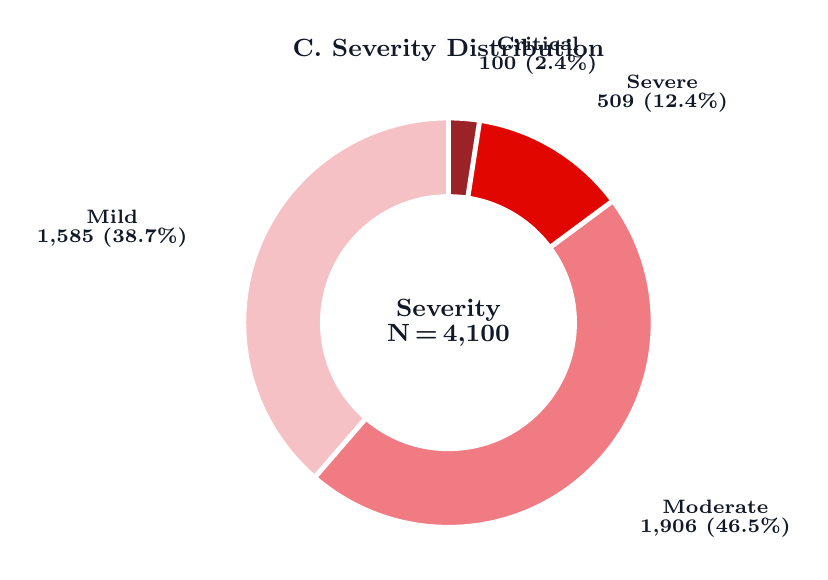
\begin{tikzpicture}
  \fill[sevCritical] (90:1.6) arc (90:81.21951219512195:1.6) -- (81.21951219512195:2.6) arc (81.21951219512195:90:2.6) -- cycle;
  \fill[sevSevere] (81.21951219512195:1.6) arc (81.21951219512195:36.52682926829268:1.6) -- (36.52682926829268:2.6) arc (36.52682926829268:81.21951219512195:2.6) -- cycle;
  \fill[sevModerate] (36.52682926829268:1.6) arc (36.52682926829268:-130.8292682926829:1.6) -- (-130.8292682926829:2.6) arc (-130.8292682926829:36.52682926829268:2.6) -- cycle;
  \fill[sevMild] (-130.8292682926829:1.6) arc (-130.8292682926829:-270.0:1.6) -- (-270.0:2.6) arc (-270.0:-130.8292682926829:2.6) -- cycle;
  \draw[white, line width=1.8pt] (0,0) circle (1.6);
  \draw[white, line width=1.8pt] (0,0) circle (2.6);
  \draw[white, line width=1.8pt] (90:1.6) -- (90:2.6);
  \draw[white, line width=1.8pt] (81.21951219512195:1.6) -- (81.21951219512195:2.6);
  \draw[white, line width=1.8pt] (36.52682926829268:1.6) -- (36.52682926829268:2.6);
  \draw[white, line width=1.8pt] (-130.8292682926829:1.6) -- (-130.8292682926829:2.6);
  \node[font=\small\bfseries, text=textdark, align=center] at (0,0) {Severity\\[-2pt]N\,=\,4,100};
  \node[anchor=west, font=\scriptsize\bfseries, text=textdark, align=center] at (0.26,3.39) {Critical\\[-1pt]100 (2.4\%)};
  \node[anchor=west, font=\scriptsize\bfseries, text=textdark, align=center] at (1.76,2.91) {Severe\\[-1pt]509 (12.4\%)};
  \node[anchor=west, font=\scriptsize\bfseries, text=textdark, align=center] at (2.31,-2.49) {Moderate\\[-1pt]1,906 (46.5\%)};
  \node[anchor=east, font=\scriptsize\bfseries, text=textdark, align=center] at (-3.19,1.19) {Mild\\[-1pt]1,585 (38.7\%)};
  \node[above, font=\small\bfseries, text=textdark] at (0,3.2) {C.\ Severity Distribution};
\end{tikzpicture}

\end{document}
